\chapter{Event reconstruction and simulation\label{sec:recosim}}

Once all the detector hits and deposits produced in a bunch collision have been recorded and stored, a sophisticated series of pattern-recognition algorithms takes these disparate data and assembles them into a picture of what actually occurred in that collision. Particle energies and trajectories are reconstructed, and particle types are identified.

Particle reconstruction algorithms are used not only for experimental data, but also for datasets of simulated physics events. Event simulation is an important component of particle physics research, as it provides a way to test data against theoretical predictions.

In this chapter, an overview is given of the standard CMS particle reconstruction procedure, and of how event reconstruction is typically performed.

\section{Particle reconstruction\label{sec:cms-reco}}
% Particle Flow (list all types of particles, focus on muons, taus, jets, MET)
Before reaching a relatively stable final state, the immediate products of the proton-proton collisions in the LHC tunnel undergo various interactions such as radiation, decays, and/or hadronization. The resulting particles travel through and interact with the material of the CMS detector, which records their passage and reconstructs their paths and energies, which are then used to identify the particles and deduce the interactions that they underwent. The set of algorithms used predominantly for particle reconstruction and identification in the CMS experiment is called Particle Flow~\cite{CMS-PAS-PFT-09-001}, often abbreviated as PF.

The basic building blocks passed to the PF algorithm are tracks and clusters. Charged particle tracks are reconstructed from hits in the silicon tracker by an iterative tracking algorithm; a similar process is done to reconstruct muon tracks in the muon detector. Track resolution is crucial for accurately determining the trajectory as each track, as inaccuracies can lead to large discrepancies in reconstructed energies. Clustering algorithms search for patterns in energy deposits in the ECAL and HCAL, to reconstruct the energies and trajectories of photons, neutral hadrons, and charged hadrons.

Once tracks and clusters are reconstructed, linking algorithms make tentative associations between these elements, based on criteria such as their closeness in distance and in energy. Track paths are extrapolated from the tracker into the ECAL and HCAL and matched to clusters if their reconstructed momenta and positions are compatible; clusters in the ECAL and HCAL are linked if the extrapolated trajectory of the ECAL cluster lies within the HCAL cluster envelope; tracks from the silicon and muon trackers are linked by performing a global $\chi^2$ fit between the two types of tracks.

Particle Flow combines all this track and cluster information from all subdetectors to build reconstructed particle objects. The abbreviation ``reco" will often be used in this dissertation to refer to reconstructed objects. Charged particle tracks linked to ECAL clusters are used to seed electron and charged hadron candidates, while ECAL and HCAL clusters that cannot be matched to any track are used to seed photon and neutral hadron candidates respectively. If the momentum from the combination of a linked muon track and silicon tracker track is compatible with the silicon tracker track momentum alone, the linked object is a PF muon candidate.

Jet clustering algorithms group electron, muon, photon, and charged or neutral hadron candidates together into jets; iterative cone techniques~\cite{1126-6708-2008-04-063} use the hardest particle or calorimeter tower in the event as a seed and builds a jet from the PF candidates in a cone around it, removes all of the jet candidates from consideration, and then moves on to find the next jet seed from the remaining candidates in the event, proceeding thus until no seeds are left. Hadronic tau decays are reconstructed from PF jets; currently the approved algorithm used by CMS is the Hadrons Plus Strips (HPS) algorithm~\cite{CMS:2011msa}, which reconstructs the decay mode of a tau based on the number of charged hadrons, neutral hadrons, and photons among the tau decay candidates. Finally, since the initial-state colliding protons have zero transverse energy, the missing transverse energy in the event is reconstructed by calculating the vector sum of the transverse energies of all reconstructed particles and taking the negative, based on the conservation of momentum.

\begin{figure}[hbtp]
  \begin{center}
    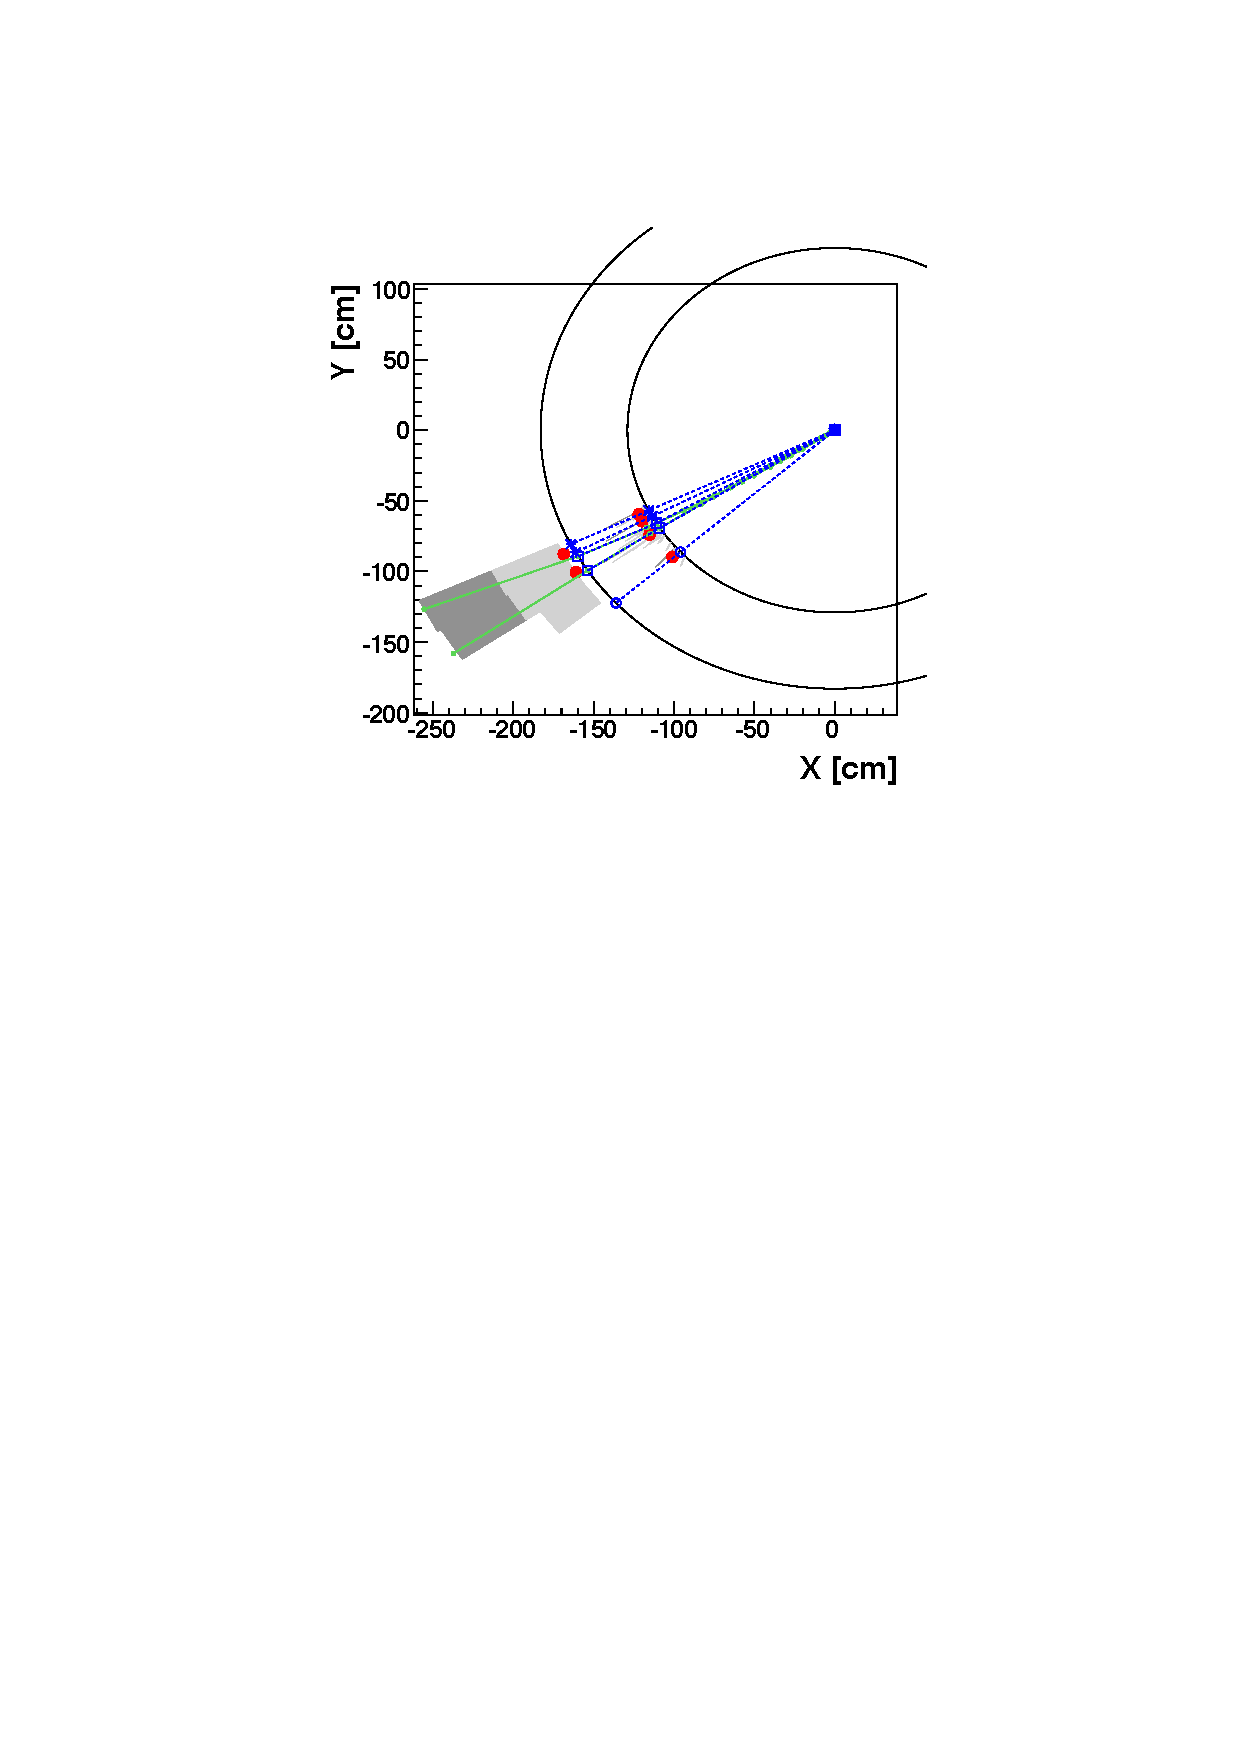
\includegraphics[width=1.0\cmsFigWidth]{figures/cms-pflow-a}
    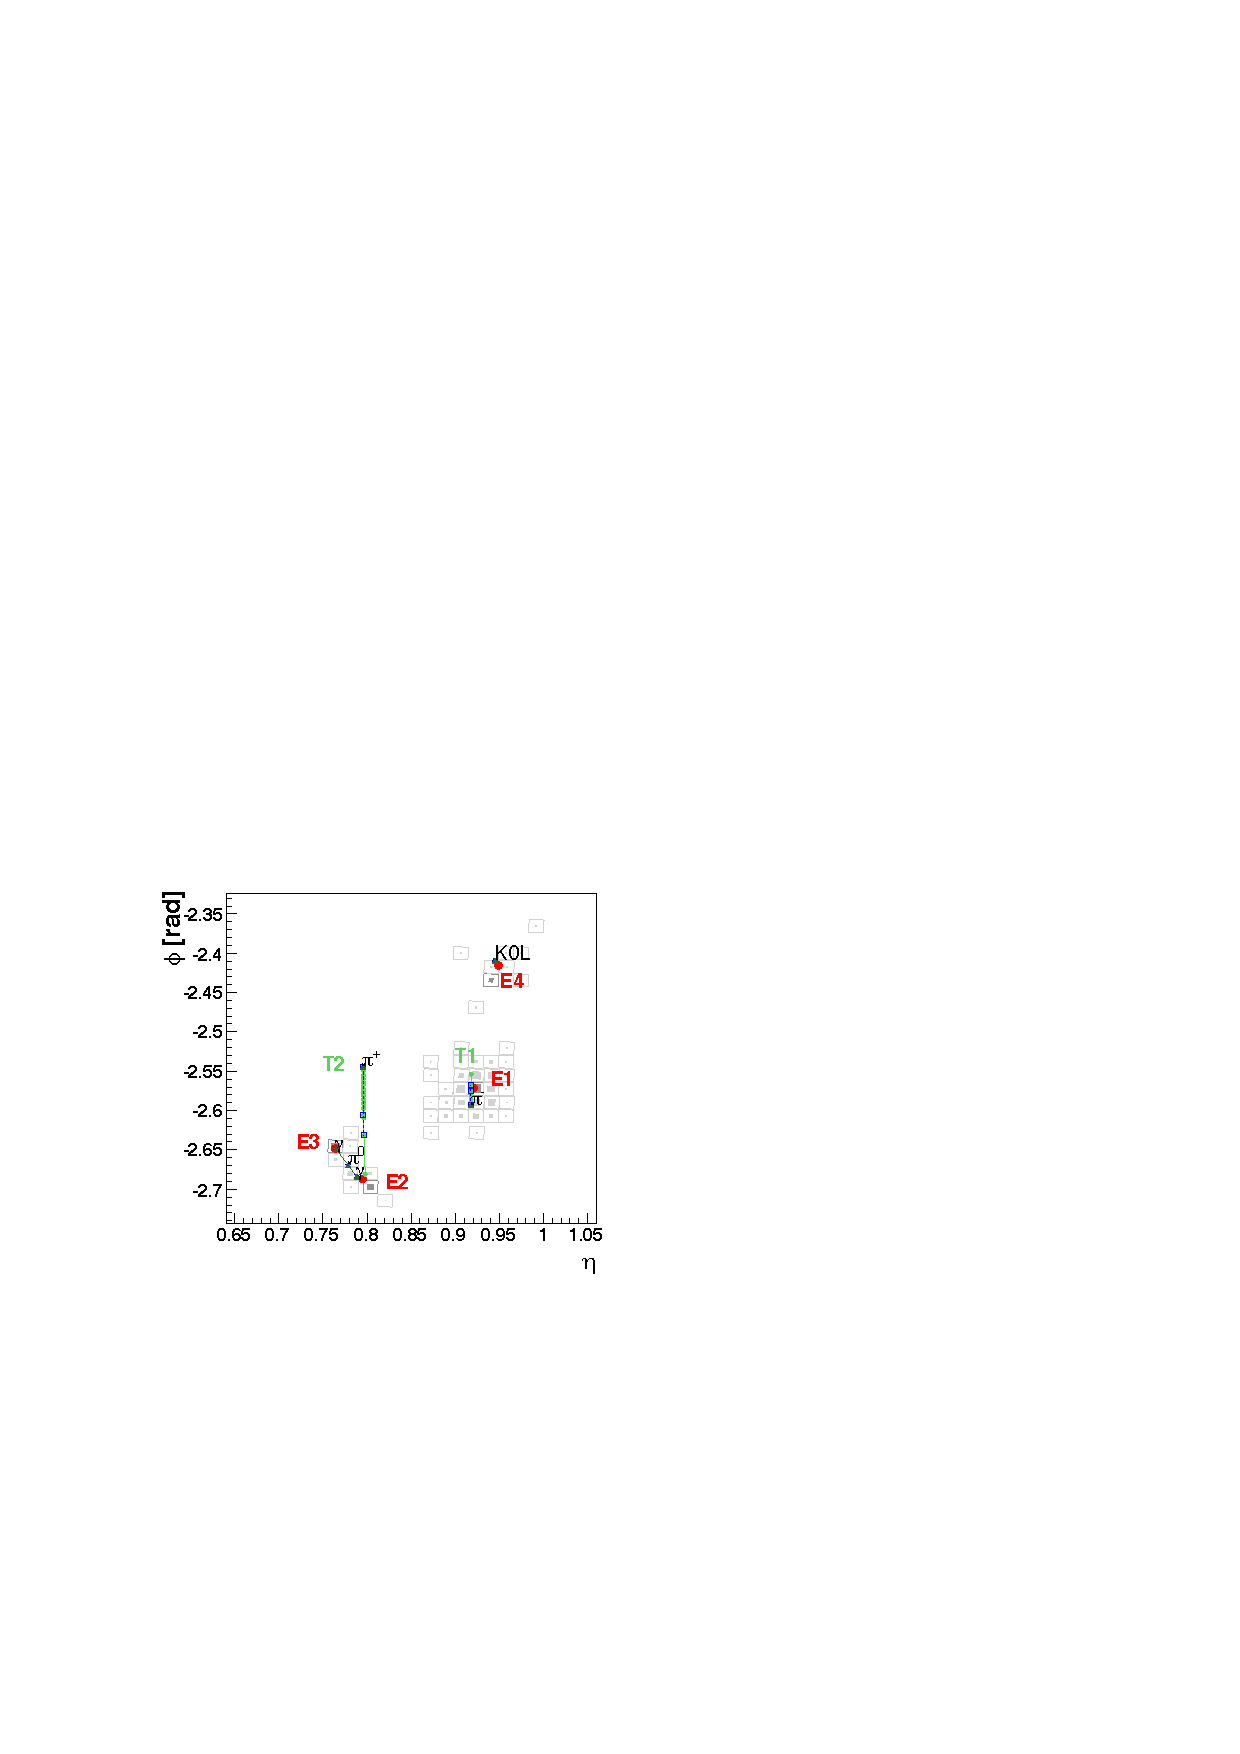
\includegraphics[width=1.0\cmsFigWidth]{figures/cms-pflow-b}
    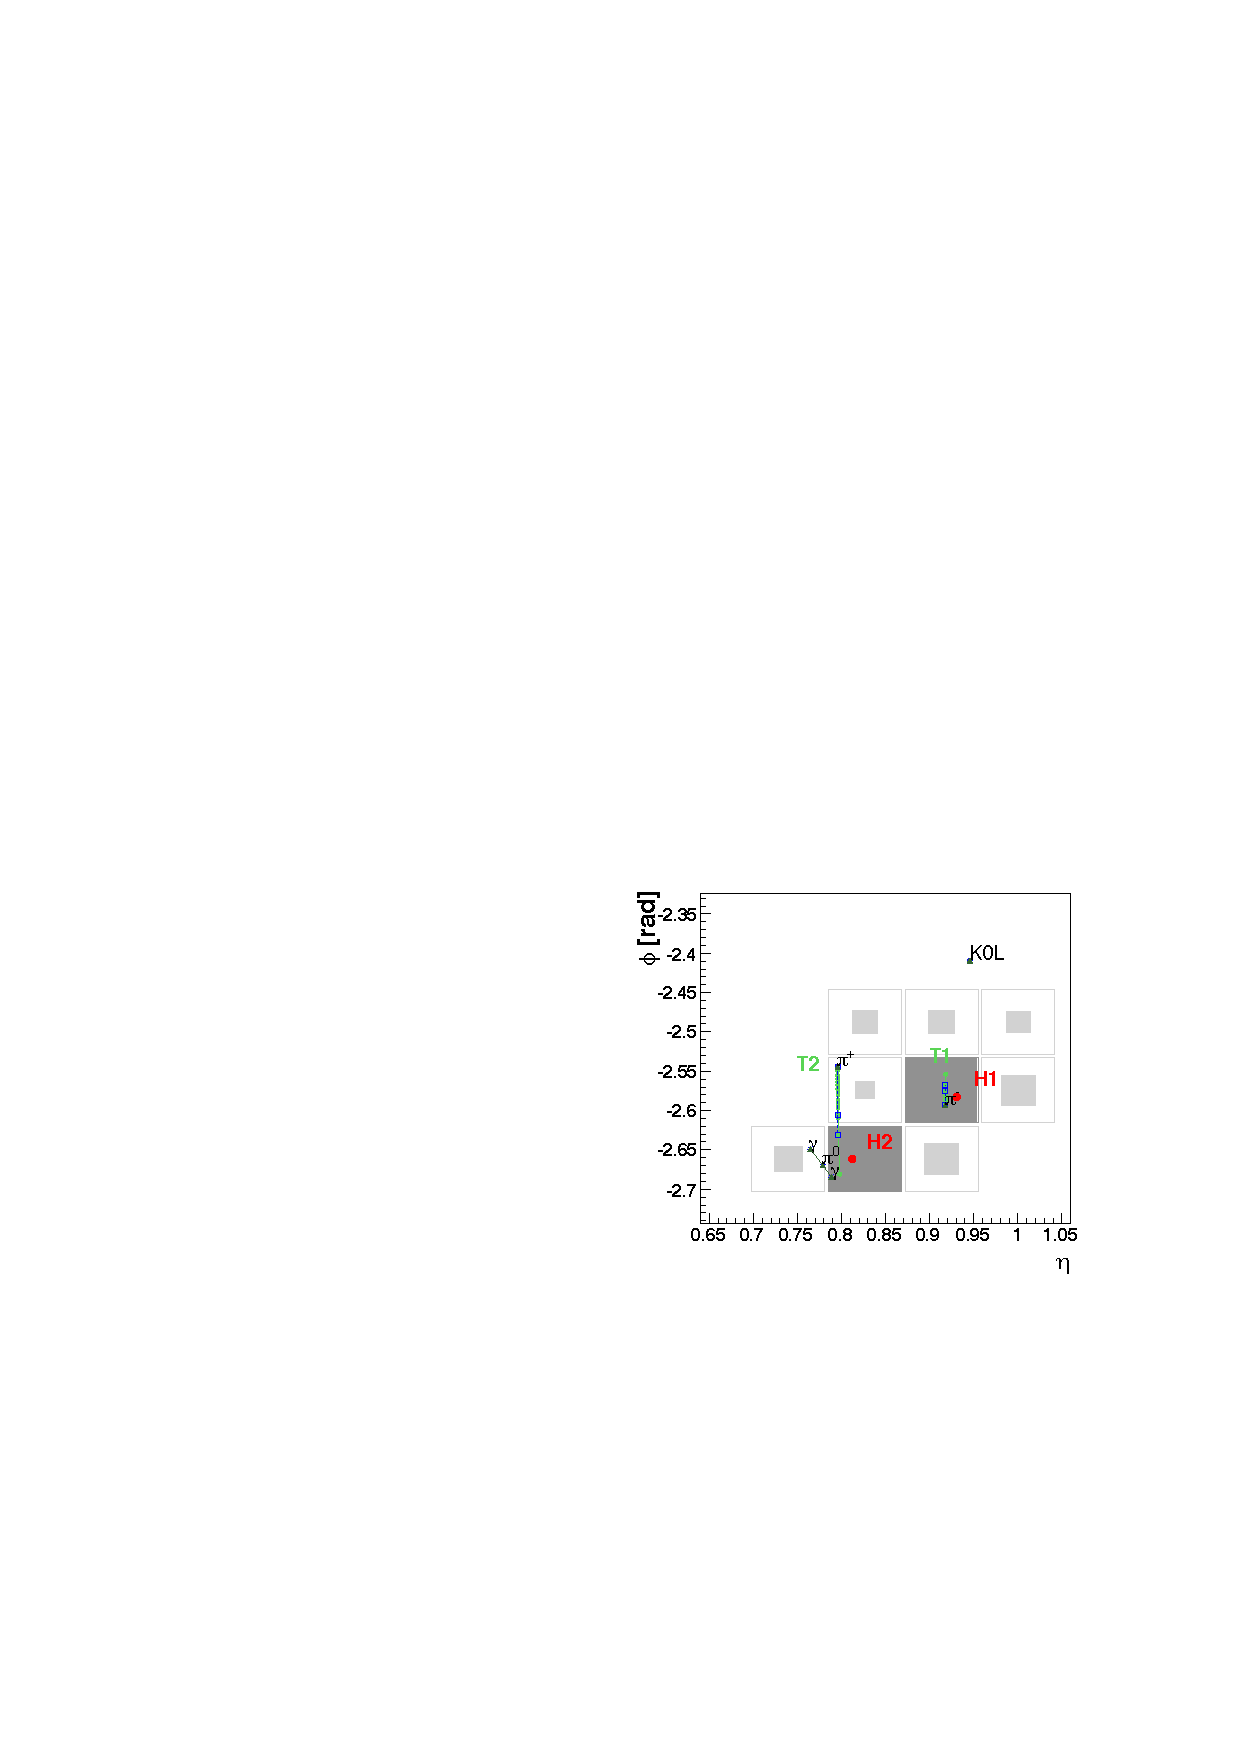
\includegraphics[width=1.0\cmsFigWidth]{figures/cms-pflow-c}
    \caption{Event display of a hadronic jet consisting of a $K^{0}_{L}$, $\pi^{+}$, $\pi^{-}$, and $\pi^{0}$, reconstructed via the Particle Flow algorithm from tracks and calorimeter deposits. The $\pi^{0}$ is detected via its decay to a pair of photons in the ECAL. Figures copied from~\cite{CMS-PAS-PFT-09-001}. (Top \cmsLeft) View in the xy plane, showing the tracks (green arcs), the ECAL and HCAL (represented by the two concentric circles), and calorimeter towers (dark and light grey for HCAL and ECAL respectively). The positions of impact of each of the four particles on the ECAL and HCAL are represented by open blue markers. (Top \cmsRight) View in the $\phi\eta$ plane for the ECAL, showing clusters reconstructed from ECAL deposits. The $K^{0}_{L}$, $\pi^{-}$, and $\pi^{0}\rightarrow\gamma\gamma$ leave four well-separated clusters E1-E4 in the ECAL, while the $\pi^{+}$ passes through without leaving an energy deposit. (Bottom) View in the $\phi\eta$ plane for the HCAL. The two charged pions are reconstructed as charged tracks T1 and T2 (green lines), pointing to HCAL clusters H1 and H2; Particle Flow associates these tracks with the respective HCAL cluster that they point to. Cluster positions are indicated by solid red dots in all three views.}
    \label{fig:cms-pflow}
  \end{center}
\end{figure}

\section{Event simulation with Monte Carlo\label{sec:cms-sim}}

Simulating particle collisions is an essential part of high-energy collider experiments. For instance, in order to determine whether actual data indicate the detection of new physics, one must know what data to expect if nothing new is occurring, so as to be able to compare collected data with predictions from the old theory; a reliable program for simulating physics processes based on known theory can provide a convenient means of obtaining a prediction for expected backgrounds. Other examples of uses for physics event simulation include calibrating the detector and testing the efficiency of its hardware and software.

The evolution of a simulated event in a collider can be broken down into two main steps: 1) modeling the particle collision and subsequent particle production, and 2) modeling the interaction of the final-state particles with the various parts of the detector, decays in flight, and the detector response. The principles behind these two aspects of event simulation will now be discussed. The physics event generation package PYTHIA~\cite{Sjostrand:2006za} and the detector simulation package GEANT4~\cite{documents:998155}, both used in the Compact Muon Solenoid (CMS) experiment, will be described as concrete examples of event simulation software. Many other packages exist that have somewhat different mechanisms, but the general principles are essentially the same.

For any particle interaction, there exists a spectrum of final states, each with its own particular amplitude for occurring. The phase space describes all the possible final states that the system can achieve; the relative probabilities for these final states are a function of the momenta and relative trajectories of the particles. The evolution of the system involves an element of randomness due to quantum mechanics; the most common technique for simulating this is is the Monte Carlo (MC) method, which uses a random number generator to sample the phase space for each simulated physics process and thus evolve of the event in a probabilistic fashion.

PYTHIA generates physics events in a series of steps. The first step is the hard scattering of the colliding initial-state particles (protons, in LHC event simulations). To generate events with the relative frequencies with which one would expect them to occur in actual colliders, the various possible reaction channels need to be weighted according to their cross-sections, which PYTHIA calculates. The initial-state particles are characterized by parton distribution functions (PDFs); even leptons, which are not partons, are described with a PDF that reflects the likelihood of photon emission by the lepton before it enters the initial hard process with a fraction $x$ of its original momentum.

Photon or gluon radiation can occur before and after the hard scattering process. PYTHIA is optimized to model $2 \rightarrow 1$ and $2 \rightarrow 2$ processes (where the numbers indicate the number of particles in the initial and final states), for which it can compute the cross-sections. However, a challenge arises in simulating radiation processes, which begin with one particle and end with two or more. Gluon radiation is especially problematic because it is governed by QCD, and for soft radiative processes -- where the radiated gluons are roughly collimated with the final-state parton -- the momentum transfer values involved are so low that strong coupling constant is large enough for processes higher than tree level to be significant, and thus amplitudes for these processes cannot be calculated perturbatively. This makes the computation of amplitudes for radiation processes extremely complicated, and PYTHIA does not perform such calculations. Instead, it uses the parton showering method to estimate the higher-order matrix elements for initial and final state radiation. Parton showering simulates the branching of one randomly-chosen ``shower initiation" parton (not necessarily the parton involved in the hard process) into a number of other partons and combining the results. PYTHIA estimates the branching probabilities for quarks, leptons, and gluons with a simplified kinematic model that is a function of the 4-momentum fraction $z$ for the branching; $1 \rightarrow 2$ decays are simulated with this model until the final-state particles in the shower reach a certain cutoff energy, below which no further radiation is simulated. The formation of jets from the beam remnants (the partons not involved directly in the hard scattering) is modeled similarly. Other event generation packages used by CMS, such as MADGRAPH~\cite{springerlink:10.1007/JHEP06(2011)128}, BlackHat, SHERPA~\cite{Berger:1177972}, and POWHEG~\cite{Alioli:2010ab}, do calculate some of the matrix elements for higher-order processes. However, due to the inherent non-perturbativeness of QCD, these calculations necessarily involve their own approximations and inaccuracies.

After the hard scattering and final-state showering, the resultant quarks and gluons must hadronize; in PYTHIA, this process is referred to as fragmentation. Often, the hadrons produced are unstable and will radiate and decay further; the series of fragmentation and decays that occur before the final state is reached are collectively termed hadronization. Again because of the non-perturbative QCD diagrams involved in the matrix elements, PYTHIA relies instead on simplified models of fragmentation based on the Lund string scheme to approximate the process.

The next step in event generation is to model the response of the detector to the particles produced in simulated collisions. At CMS, GEANT4 is used to model the trajectories of final-state particles and their interactions with the parts of the detector in their path, and the way in which the detector elements register and record the particles that pass through them.

The geometry of the detector -- the material composition, positions, dimensions, etc. of its components (both sensitive elements and structural supports) -- must be specified in the simulation program. Monte Carlo methods are used to model the interaction of particles with the detector components. The rate of energy loss per unit distance is determined by the medium's chemical composition and by the type of interaction involved in the energy deposition, which depends on on the particle's energy; for different particle energies, processes such as ionization (governed by the Bethe-Bloch equation) and bremsstrahlung occur with different relative probabilities, characterized by a mean free path (radiation length for bremsstrahlung, and hadronic interaction length for strong interactions)~\cite{Tavernier:1172614}.

When final-state particles emerge from a simulated collision, GEANT4 simulates each particle's trajectory step-by-step through the detector volume, evolving it under the influence of electromagnetic fields and also via its interactions with the materials that it passes through. For each step that a particle makes, all possible types of interactions with the detector material are considered, and cross-sections are computed for all of them; the probability and spacetime step-lengths for each interaction are then calculated, and the smallest step-length is selected; the spacetime position and kinematic properties of the particle are then updated and the particle is ready for the next step to be simulated. Simulated hits in the detector are interpreted by algorithms and clustered together to reconstruct the kinematics and paths of particles in the event.

The detector's efficiency is the frequency with which it correctly records and reconstructs events. To have a realistic picture of the detector's performance, its finite resolution and inefficiencies must be included in the simulation. For any given physics search, the detector efficiency can be considered as a combination of two main factors. The first is the acceptance -- the probability that a simulated particle passing through the simulated detector will be reconstructed. This depends on the geometry of the detector -- where its components and dead space are located -- and on the physics that produced that particle, which determines the probability that it will be produced with the right kinematic properties (e.g., momentum and scattering angle) to pass through the active part of the detector and be recorded. The other factor -- the reconstruction efficiency -- is the probability that the track will be reconstructed in a way that accurately represents the actual particle and its path. This depends on whether the particle satisfies the triggering criteria, and on the selection criteria used to filter out background events. The total efficiency is the product of the acceptance and the reconstruction efficiency~\cite{CMS:2010mua}~\cite{Chatrchyan:2012rga}.

Detector acceptance can be modelled in the GEANT simulation by passing it a database of the calibration constants and detector element efficiencies measured at CMS in calibration studies; these detector conditions are used to correct the representation of particle interactions with individual detector components and better simulate their efficiencies or inefficiencies.

Modelling reconstruction efficiencies is best illustrated by an example. The efficiency for simulated muons to pass a particular HLT path may differ from that of actual muons in data, due to the imperfection of modelling the detector acceptance. The discrepancy may vary with the trigger muon's $p_T$, $\eta$, and other kinematic parameters. Thus, in order to make the simulated HLT efficiency agree better with actual data, official studies are done at CMS to measure data/MC scale factors as a function of trigger muon $p_T$, $\eta$, and other important kinematic parameters that these discrepancies may depend on. Then, when an HLT filter is applied to a dataset of MC events, each event is weighted by the appropriate scale factor, depending on the $p_T$, $\eta$, etc. of the trigger muon. Scale factors are calculated for basic ID selections on reconstructed objects at CMS and are thus used for weighting the events used in MC datasets in order to represent the effect of reconstruction inefficiencies.
